\documentclass[11pt, a4paper]{article}

\title{
KumoLang:
A Formal Verification Framework for Cheesecake Synthesis
\thanks{The authors are having a hard time coping with their end-of-terms so some features are still TODO. Please be patient.}
\thanks{
This is a joke paper. However, KumoLang is a language that actually works, and if one does not mind expressing recipes in a Lisp-like syntax, it is entirely suitable for daily cheesecake synthesis workflows.
}
\thanks{
Portions of this manuscript were generated with the assistance of AI tools. The language design, operational semantics, and formalization were developed by the authors. While the presentation is intentionally comedic, the underlying formal methods are genuine.
}
\thanks{
The authors thank Kumo for an excellent APCSA course.
}
\thanks{
The authors thank KumoKumo for producing the Basque cheesecakes that inspired this work.
}
\thanks{
KumoLang is a purely noncommercial, open-source, academic parody and educational experiment. It is developed entirely for non-profit pedagogical purposes, research exploration in programming language theory (PLT), and personal recreation. No revenue, commercial services, or physical products are associated with this project. It is a standalone project and is not affiliated with, authorized, maintained, sponsored, or endorsed by, or in any way officially connected to the pastry brand KumoKumo, any of its affiliates, or any other entity or individual utilizing the name "Kumo".
}
}
\author{
  Sean L. \\
  \and
  Thomas W. \\
  \and
  Eric Y. \\
  \and
  Jack Z. \\
  \and
  Hachimi R. \\
}
\usepackage{amsmath, amssymb, amsthm}
\usepackage{listings}
\usepackage{algorithm}
\usepackage{algpseudocode}
\usepackage{semantic}
\usepackage{tikz}
\usepackage{hyperref}
\usepackage{graphicx}
\usepackage{pdflscape}

\newtheorem{theorem}{Theorem}
\newtheorem{lemma}[theorem]{Lemma}
\newtheorem{corollary}[theorem]{Corollary}

\begin{document}
\maketitle
\begin{abstract}
    We present \textbf{KumoLang}, a purely imperative specification language and verification framework that formalizes culinary execution procedures through linear state transitions and structural correctness-by-construction, and an proof-of-concept verification engine in Rust (\url{https://github.com/makabaka1880/kumolang}). Unlike traditional stateful architectures that rely on decoupled static analysis or complex reference counting, the operational semantics of KumoLang inherently guarantee a well-formed, acyclic dependency trace during runtime evaluation. We formalize the core syntax and execution state through a list-monad architecture: raw components are lifted into isolated container types via a monadic \text{\texttt{prep}} constructor, combined symmetrically via an endomorphic \text{\texttt{pour}} operator, and transitioned across distinct nominal domains using a type-lifting \text{\texttt{pour-out}} functor. Because the structural rules of the calculus strictly forbid invalid resource configurations, ill-formed physical configurations—such as domain cross-contamination or unbound variable references—are rendered completely unrepresentable. This tight coupling of language semantics and safety invariants allows the framework to enforce absolute domain boundaries natively, ensuring the deterministic, verified synthesis of a target KumoKumo Basque pastry specification with zero compilation or runtime verification overhead.
\end{abstract}

% --- SECTION 1: INTRODUCTION ---
\section{Introduction}
In his foundational work \emph{Tractatus Logico-Philosophicus}, Ludwig Wittgenstein famously asserted, ``The world is everything that is the case. The world is the totality of facts, not of things'' \cite{wit}. If we extend this analytical framework to the physical bounds of the culinary arts, we encounter a profound systemic failure in modern procedural tracking. The modern kitchen is not a loose collection of macroscopic things (e.g., cheese, eggs, vessels); it is a rigorous totality of state-based facts, thermodynamic boundaries, and irreversible substructural transformations.

Traditionally, the formal verification of physical procedures has been severely neglected by the programming language theory (PLT) community. This oversight has left the domain of recipe analysis primarily to coarse natural language processing (NLP) heuristics and machine learning dependency graphs designed for general commonsense reasoning \cite{commonsense}. These stochastic methods are fundamentally inadequate. They treat a physical sequence as a relaxed recommendation rather than what it truly is: a stateful, resource-bounded program. In a physical environment, resources are consumed linearly, and state transformations are destructive and non-monotonic. An egg, once emulsified into a dairy matrix, cannot be recovered via structural weakening or contraction.

To rectify this foundational gap, we introduce \textbf{KumoLang}, a purely imperative specification language and verification framework engineered to formalize the synthesis of complex multi-component pastries—specifically optimized for a localized compilation target of a KumoKumo Basque cheesecake. Unlike traditional verification platforms that require upfront static linting passes to check resource safety, the structural semantics of KumoLang inherently guarantee a well-formed directed acyclic graph (DAG) of physical dependencies directly during linear statement evaluation. By mapping execution to a strict sequential list-monad algebra, the small-step operational evaluation of an un-nested program naturally achieves a state of \emph{Correctness-by-Construction}: raw mixtures are instantiated as isolated, generative nominal types, which are subsequently manipulated as linear container assets. The resulting abstract semantic trace renders invalid physical states completely unrepresentable, ensuring the deterministic and verified synthesis of the target pastry specification with zero runtime overhead.

The remainder of this paper is organized as follows. Section~2 presents the abstract syntax and small-step operational semantics of KumoLang, formalizing its core monadic operators and the structural invariants they enforce. Section~3 introduces the Kumo Verification Engine, walking through a complete trace evaluation for a canonical cheesecake synthesis program and presenting the resulting provenance DAG. Section~4 concludes, Section~5 outlines directions for future work, and Section~6 surveys related work.

\section{Syntax and Abstract Architecture}

We now formalize the core calculus that underpins the guarantees outlined above. The language utilizes an S-Expression syntax restricted to variable identifiers for operational arguments, structurally enforcing a clear line of resource custody. We begin with the formal grammar, then define the semantic domains over which evaluation operates, and finally present the small-step operational semantics that constitute the heart of the verification framework.
% --- SUBSECTION: FORMAL GRAMMAR ---
\subsection{Formal Grammar}
Let $x, y, z \in \text{Var}$ range over variable identifiers tracking active mixtures or container states. A KumoLang program $P$ consists of a sequentially composed chain of statements $s$, defined inductively by the following abstract syntax:

\[
\begin{array}{rcll}
P & ::= & s & \text{(Instruction)} \\
  & \mid  & s \;;\; P & \text{(Sequence)} \\
[1.5ex]
s & ::= & \text{\texttt{skip}} & \text{(Stasis)} \\
  & \mid  & x \leftarrow \text{\texttt{new-mixture}}() & \text{(Domain allocation)} \\
  & \mid  & y \leftarrow \text{\texttt{prep}}(x) & \text{(Lift mixture $x$ to container $y$)} \\
  & \mid  & y \leftarrow \text{\texttt{pour}}(y, z) & \text{(Merge container $z$ into container $y$)} \\
  & \mid  & z \leftarrow \text{\texttt{pour-out}}(y, x) & \text{(Type casting: lift container $y$ into domain $x$)} \\
\end{array}
\]


\subsection{Semantic Domains}
Having specified the syntactic forms, we now define the semantic domains over which program evaluation operates. Unlike conventional general-purpose programming languages designed for value transformation or numerical computation, KumoLang is a domain-specific specification language. Its operational semantics do not model a traditional abstract machine; rather, they formally characterize the evolution of valid structural relationships and resource tracking. An execution trace represents a sequence of logical validations proving that a physical process is structurally coherent.

We define the semantic domains to track nominal mixture scopes and container configurations. Let $\mathcal{M}$ be a countable set of generative mixture domain tokens, and $\text{Var}$ be the set of variable identifiers. 

\[
\begin{array}{rclr}
m &\in& \mathcal{M} & \text{(Nominal Mixture Identifiers)} \\
L &\in& \mathcal{L}_m = \text{List}(m) & \text{(Structural History List Domain)} \\
\sigma &\in& \text{Store} = \text{Var} \to (\mathcal{M} \cup \mathcal{L}_m) & \text{(Structural Environment State)} \\
\end{array}
\]

When a variable identifier is resolved in the environment store $\sigma$, it maps to one of two structural categories:
\begin{itemize}
    \item \textbf{Mixture Labels ($m \in \mathcal{M}$):} Act as a strict type-level boundary. Objects belonging to separate mixture universes cannot cross-contaminate.
    \item \textbf{Container Configurations ($L \in \mathcal{L}_m$):} Represent the physical state of a vessel, formalized as a list tracking the chronological history log of components poured into it.
\end{itemize}

\subsection{Small-Step Operational Semantics}
With the store model in place, we now define the evaluation relation that governs program execution. A state configuration is defined as a pair $\langle P, \sigma \rangle$, where $P$ is the remaining program sequence and $\sigma$ is the current environmental store. The structural evaluation relation $\langle P, \sigma \rangle \to \langle P', \sigma' \rangle$ defines a single step of structural validation. We present the inference rules for each statement form below. 

\[
\inference[\text{Stasis}]{}
{\langle \text{\texttt{skip}} ; P \;,\; \sigma \rangle \nrightarrow }
\]

\[
\inference[\text{Domain-Alloc}]{m \notin \text{img}(\sigma)}
{\langle x \leftarrow \text{\texttt{new-mixture}}() ; P \;,\; \sigma \rangle \to \langle P \;,\; \sigma[x \leftarrow m] \rangle}
\]

\[
\inference[\text{Ing-Prep}]{\sigma(x) = m}
{\langle y \leftarrow \text{\texttt{prep}}(x) ; P \;,\; \sigma \rangle \to \langle P \;,\; \sigma[y \leftarrow [m]] \rangle}
\]

\[
\inference[\text{Pour-In}]{\sigma(y) = L_1 \in \mathcal{L}_m \quad \sigma(z) = L_2 \in \mathcal{L}_m}
{\langle y \leftarrow \text{\texttt{pour}}(y, z) ; P \;,\; \sigma \rangle \to \langle P \;,\; \sigma[y \leftarrow L_1 \mathbin{+\mkern-10mu+} L_2] \rangle}
\]

\[
\inference[\text{Pour-Out}]{\sigma(y) = L_1 \in \mathcal{L}_m \quad \sigma(x) = m_{\text{target}}}
{\langle z \leftarrow \text{\texttt{pour-out}}(y, x) ; P \;,\; \sigma \rangle \to \langle P \;,\; \sigma[y \leftarrow [], \; z \leftarrow [m_{\text{target}}]] \rangle}
\]

\section{The Kumo Verification Engine}

The operational semantics of Section~2 define, in principle, what constitutes a valid culinary execution. In practice, however, verifying that a given program actually produces the desired pastry requires a concrete evaluation engine. The Kumo Verification Engine realizes this by computing small-step reduction sequences from an initial program-store configuration and extracting the resulting dependency trace as a certifiable artifact. We now illustrate this process end-to-end.

\subsection{Provenance DAG Generation}
Because KumoLang permits only forward construction of culinary artifacts, the provenance graph associated with any execution trace is guaranteed to be a directed acyclic graph (DAG). Each vertex corresponds to a variable-binding event occurring during evaluation, while each directed edge records a provenance relation between two bindings. Intuitively, an edge $(u,v) \in E$ indicates that the value bound at $v$ was derived, directly or indirectly, from the value bound at $u$.

The provenance graph is constructed incrementally during evaluation. Operations introduce fresh bindings and establish provenance edges from their operands to the newly created binding. For example, a \texttt{prep} operation introduces a new ingredient binding and records a provenance edge from the source mixture to the ingredient. Likewise, a \texttt{pour} operation introduces a new container binding and records provenance edges from each source container to the resulting container. Finally, a \texttt{pour-out} operation introduces a new container binding whose provenance depends on both the source container and the target mixture.

Acyclicity follows from the operational semantics. Every transition introduces a fresh binding that may depend only on bindings already present in the environment. Consequently, all provenance edges are directed from older bindings to newer bindings, and no operation can introduce a path from a binding back to itself. The resulting graph therefore admits a topological ordering induced by the evaluation trace.

The provenance extraction process operates on a graph state

\[
G = \langle V,E,\tau,\lambda,\iota\rangle
\]

where $V$ is the set of provenance vertices, $E \subseteq V \times V$
is the set of directed provenance edges, $\tau : V \to \{\mathsf{Mixture}\} \cup \{\mathsf{Ingredient}(v) \mid v \in V\} \cup \{\mathsf{Container}(v) \mid v \in V\}$ assigns a parametric semantic
kind to each vertex (an ingredient or container is always tagged with the mixture vertex it belongs to), $\lambda$ assigns a human-readable label, and

\[
\iota : \mathcal N \rightharpoonup V
\]

maps identifiers to their most recent provenance vertex.

The provenance extraction relation

\[
\langle P,G\rangle \rightsquigarrow \langle P',G'\rangle \cup G'
\]

is evaluated in parallel with the operational semantics. The complete algorithm is provided in the appendix \ref{prov-gen}.

\subsection{Trace Evaluation}
We demonstrate the evaluation of a simple KumoLang program that synthesizes a basic cheesecake specification. Consider the following program, which allocates two mixture domains (a base mixture for ingredients and a baking mixture for the final product), prepares two ingredients from the base domain, combines them via a pour, and finally transitions the combined container into the baking domain. 
\[
\begin{array}{l}
\text{BaseMix} \leftarrow \text{\texttt{new-mixture}}() \;;\; \\
\text{BakeMix} \leftarrow \text{\texttt{new-mixture}}() \;;\; \\
c_{\text{cheese}} \leftarrow \text{\texttt{prep}}(\text{BaseMix}) \;;\; \\
c_{\text{sugar}} \leftarrow \text{\texttt{prep}}(\text{BaseMix}) \;;\; \\
c_{\text{bowl}} \leftarrow \text{\texttt{pour}}(c_{\text{cheese}}, c_{\text{sugar}}) \;;\; \\
c_{\text{cake}} \leftarrow \text{\texttt{pour-out}}(c_{\text{bowl}}, \text{BakeMix}) \;;\; \\
\text{\texttt{skip}}
\end{array}
\]
We evaluate the operational semantics on this program by applying the inference rules of Section~2.3. Let the initial store be the empty environment:

\[
\sigma_0 = \emptyset.
\]

The execution proceeds through a sequence of small-step reductions.

\begin{align*}
\langle P_0,\sigma_0\rangle
&\to
\langle P_1,\sigma_1\rangle
&& \textsc{Domain-Alloc}
\\
&\to
\langle P_2,\sigma_2\rangle
&& \textsc{Domain-Alloc}
\\
&\to
\langle P_3,\sigma_3\rangle
&& \textsc{Ing-Prep}
\\
&\to
\langle P_4,\sigma_4\rangle
&& \textsc{Ing-Prep}
\\
&\to
\langle P_5,\sigma_5\rangle
&& \textsc{Pour-In}
\\
&\to
\langle P_6,\sigma_6\rangle
&& \textsc{Pour-Out}
\\
&\to
\langle \texttt{skip},\sigma_6\rangle
&& \textsc{Stasis}
\end{align*}

where the intermediate stores, obtained by applying the corresponding semantic rule at each step, are given by

\[
\sigma_1
=
\{
\text{BaseMix} \mapsto m_1
\},
\]

\[
\sigma_2
=
\{
\text{BaseMix} \mapsto m_1,
\text{BakeMix} \mapsto m_2
\},
\]

\[
\sigma_3
=
\sigma_2
\bigl[
c_{\mathrm{cheese}}
\mapsto
[m_1]
\bigr],
\]

\[
\sigma_4
=
\sigma_3
\bigl[
c_{\mathrm{sugar}}
\mapsto
[m_1]
\bigr],
\]

\[
\sigma_5
=
\sigma_4
\bigl[
c_{\mathrm{bowl}}
\mapsto
[m_1,m_1]
\bigr],
\]

\[
\sigma_6
=
\sigma_5
\bigl[
c_{\mathrm{bowl}}
\mapsto
[],
\;
c_{\mathrm{cake}}
\mapsto
[m_2]
\bigr].
\]

The final configuration certifies the successful construction of a cheesecake artifact within the baking domain $m_2$: variable $c_{\mathrm{cake}}$ is bound to the singleton history list $[m_2]$, confirming that the combined contents of the bowl have been correctly transitioned into the target baking domain. Meanwhile, $c_{\mathrm{bowl}}$ has been drained to the empty list $[]$, reflecting the physical reality that the bowl is now empty—its contents having been irreversibly transferred.

\subsection{Provenance Extraction}
While the operational trace above validates that each resource configuration is structurally coherent, the provenance extraction relation $\rightsquigarrow$ (defined formally in Appendix~\ref{prov-gen}) runs in lockstep with the evaluation, constructing a directed acyclic graph that records the dependency structure of the entire synthesis. Each small-step reduction induces a corresponding provenance transition $\langle P, G\rangle \rightsquigarrow \langle P', G'\rangle$ that augments the graph state $G = \langle V, E, \tau, \lambda, \iota\rangle$ with fresh vertices and edges.

Applying the provenance rules to our example program yields the DAG shown in Figure~\ref{fig:provenance-dag}. The graph contains six vertices reflecting the semantic role of each binding: two mixture vertices ($v_1$, $v_2$) created by \texttt{new-mixture}; two ingredient vertices ($v_3$, $v_4$) created by \texttt{prep}, each parametric to the base mixture $v_1$ (i.e., $\tau(v_3) = \tau(v_4) = \mathsf{Ingredient}(v_1)$); one container vertex ($v_5$) created by \texttt{pour}, parametric to $v_1$ (i.e., $\tau(v_5) = \mathsf{Container}(v_1)$); and one container vertex ($v_6$) created by \texttt{pour-out}, parametric to the target baking mixture $v_2$ (i.e., $\tau(v_6) = \mathsf{Container}(v_2)$). The six directed edges encode the full provenance chain: ingredients $v_3$ and $v_4$ each derive from the base mixture $v_1$; the combined container $v_5$ depends on both $v_3$ and $v_4$; and the final container $v_6$ depends on both the drained container $v_5$ and the target baking mixture $v_2$. The acyclicity of the graph follows directly from the operational semantics: every provenance rule introduces edges only from pre-existing vertices to a freshly allocated vertex, so no cycle can form. The resulting graph therefore admits a topological ordering induced by the evaluation trace—in this case, $v_1 \prec v_2 \prec v_3 \prec v_4 \prec v_5 \prec v_6$.

\begin{figure}[htbp]
\centering
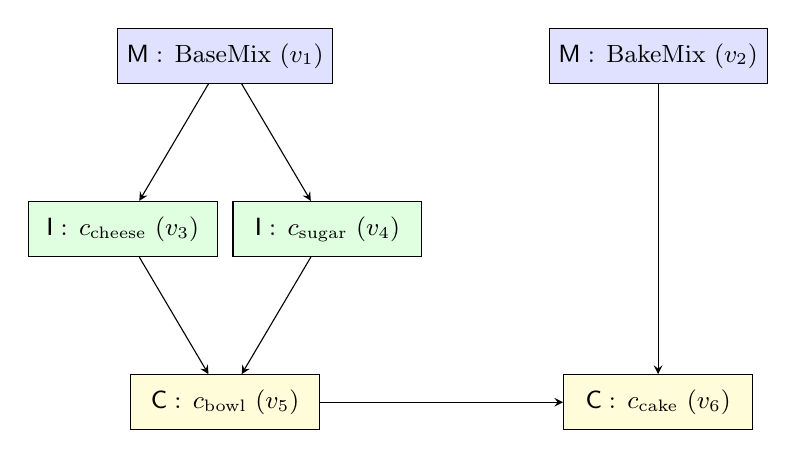
\begin{tikzpicture}[
  >=stealth,
  every node/.style={draw, minimum width=2.4cm, minimum height=0.7cm, font=\small},
  mixture/.style={fill=blue!12},
  ingredient/.style={fill=green!12},
  container/.style={fill=yellow!15},
  every edge/.style={draw, ->, >=stealth, thick},
]
  % Row 1: Mixtures
  \node[mixture] (m1) at (0,0) {$\mathsf{M}$\;: BaseMix ($v_1$)};
  \node[mixture] (m2) at (5.5,0) {$\mathsf{M}$\;: BakeMix ($v_2$)};

  % Row 2: Ingredients (from prep)
  \node[ingredient] (cch) at (-1.3,-2.2) {$\mathsf{I}$\;: $c_{\mathrm{cheese}}$ ($v_3$)};
  \node[ingredient] (csu) at (1.3,-2.2) {$\mathsf{I}$\;: $c_{\mathrm{sugar}}$ ($v_4$)};

  % Row 3: Container (from pour)
  \node[container] (cbw) at (0,-4.4) {$\mathsf{C}$\;: $c_{\mathrm{bowl}}$ ($v_5$)};

  % Row 3 (right): Container (from pour-out)
  \node[container] (cck) at (5.5,-4.4) {$\mathsf{C}$\;: $c_{\mathrm{cake}}$ ($v_6$)};

  % Edges
  \draw[->] (m1) -- (cch);
  \draw[->] (m1) -- (csu);
  \draw[->] (cch) -- (cbw);
  \draw[->] (csu) -- (cbw);
  \draw[->] (cbw) -- (cck);
  \draw[->] (m2) -- (cck);
\end{tikzpicture}
\caption{Provenance DAG extracted from the example cheesecake synthesis program. Vertex colors and labels indicate provenance kind: $\mathsf{M}$ = Mixture, $\mathsf{I}$ = Ingredient (parametric to parent mixture), $\mathsf{C}$ = Container (parametric to parent mixture). Edges are directed from source to derived binding, encoding the full dependency chain from domain allocation through to the final product. The graph is guaranteed acyclic by the operational semantics: every rule introduces edges only from pre-existing vertices to a freshly allocated vertex.}
\label{fig:provenance-dag}
\end{figure}

The provenance graph serves as a certifiable artifact of correct synthesis: it demonstrates not only that the program ran without error, but that every intermediate binding is traceable to a valid domain allocation, that no cross-contamination occurred (containers $v_3$ and $v_4$ share the same mixture ancestor $v_1$), and that the final product $v_6$ correctly depends on both the combined bowl contents and the target baking domain.

\subsection{Implementation}
The trace extraction and graph construction procedures described above have been realized in a prototype implementation. A Rust implementation of the Kumo Verification Engine is available at \url{https://github.com/makabaka1880/kumolang}. The engine accepts programs in a concrete S-expression syntax (detailed in Appendix~\ref{conc-synt}), computes the full small-step reduction sequence, and outputs the corresponding provenance graph in both human-readable and machine-readable (JSON) formats. The implementation enriches the formal provenance model of Appendix~\ref{prov-gen} with additional intermediate vertices—for instance, \texttt{prep} generates both a container vertex and an ingredient vertex linked by an intermediate edge—yielding a finer-grained dependency trace than the abstract rules prescribe. This additional resolution is semantically conservative: the coarser formal graph can be recovered by contracting each ingredient--container chain into a single vertex.

\section{Conclusion}

We have presented KumoLang, a purely imperative specification language whose operational semantics provide correctness-by-construction guarantees for physical culinary procedures. By encoding resource manipulation as a list-monad algebra over nominal mixture domains, the framework renders invalid configurations—cross-contamination, unbound references, and structural cycles—completely unrepresentable. The Kumo Verification Engine demonstrates that these guarantees can be realized in practice, producing certifiable provenance graphs from small-step reduction traces with zero runtime verification overhead. While the current framework is scoped to linear, non-recursive pastry synthesis, the underlying semantic architecture is general and invites extension to more expressive culinary settings.

\section{Future Work}

Several extensions remain unexplored. First, we intend to extend KumoLang with support for recursive pastry generation and higher-order baking combinators. Second, we plan to investigate distributed compilation across multiple ovens. Finally, we hope to formalize a dependent type system capable of statically ruling out crust formation.

\section{Related Work}
To our knowledge, KumoLang is the first formal verification framework designed specifically for culinary procedure synthesis, particularly in the domain of Basque cheesecake preparation. Prior work on recipe representation has focused primarily on natural-language parsing and commonsense knowledge graphs~\cite{commonsense}, which model cooking actions as relaxed recommendations rather than as resource-linear programs with formal safety guarantees. In the broader PLT literature, substructural type systems (e.g., linear and affine types) have been applied to resource management, and monadic embeddings have been used to structure effectful computations; KumoLang adapts these techniques to the novel domain of physical culinary state, demonstrating that correctness-by-construction is achievable even for pastry specification.

\appendix

\begin{landscape}
    
\section{Provenance Generation}
\label{prov-gen}
    \[
    \inference[\text{Stasis-Prov}]{}
    {
    \langle
    \text{\texttt{skip}} ; P \;,\;
    \langle V,E,\tau,\lambda,\iota\rangle
    \rangle
    \rightsquigarrow
    \langle V,E,\tau,\lambda,\iota\rangle
    }
    \]

    \[
    \inference[\text{Domain-Alloc-Prov}]
    {
    v \notin V
    }
    {
    \left\langle
    x \leftarrow \text{\texttt{new-mixture}}() ; P \;,\;
    \langle V,E,\tau,\lambda,\iota\rangle
    \right\rangle
    \rightsquigarrow
    \left\langle
    P \;,\;
    \left\langle
    V \cup \{v\},
    E,
    \tau[v \mapsto \textsf{Mixture}],
    \lambda[v \mapsto x],
    \iota[x \mapsto v]
    \right\rangle
    \right\rangle
    }
    \]
    
    \[
    \inference[\text{Ing-Prep-Prov}]
    {
    \iota(x)=v_m
    \qquad
    \tau(v_m)=\mathsf{Mixture}
    \qquad
    v_i \notin V
    }
    {
    \left\langle
    y \leftarrow \text{\texttt{prep}}(x) ; P \;,\;
    \langle V,E,\tau,\lambda,\iota\rangle
    \right\rangle
    \rightsquigarrow
    \left\langle
    P \;,\;
    \left\langle
    V \cup \{v_i\},
    E \cup \{(v_m,v_i)\},
    \tau[v_i \mapsto \mathsf{Ingredient}(v_m)],
    \lambda[v_i \mapsto y],
    \iota[y \mapsto v_i]
    \right\rangle
    \right\rangle
    }
    \]
    
    \[
    \inference[\text{Pour-In-Prov}]
    {
    \iota(y)=v_1
    \qquad
    \iota(z)=v_2
    \qquad
    \tau(v_1)=\mathsf{Container}(v_m)
    \qquad
    \tau(v_2)=\mathsf{Container}(v_m)
    \qquad
    v_c \notin V
    }
    {
    \left\langle
    c \leftarrow \text{\texttt{pour}}(y,z) ; P \;,\;
    \langle V,E,\tau,\lambda,\iota\rangle
    \right\rangle
    \rightsquigarrow
    \left\langle
    P \;,\;
    \left\langle
    V \cup \{v_c\},
    E \cup \{(v_1,v_c),(v_2,v_c)\},
    \tau[v_c \mapsto \mathsf{Container}(v_m)],
    \lambda[v_c \mapsto c],
    \iota[c \mapsto v_c]
    \right\rangle
    \right\rangle
    }
    \]
    
    \[
    \inference[\text{Pour-Out-Prov}]
    {
    \iota(y)=v_c
    \qquad
    \iota(x)=v_m
    \qquad
    \tau(v_m)=\mathsf{Mixture}
    \qquad
    v_o \notin V
    }
    {
    \left\langle
    z \leftarrow \text{\texttt{pour-out}}(y,x) ; P \;,\;
    \langle V,E,\tau,\lambda,\iota\rangle
    \right\rangle
    \rightsquigarrow
    \left\langle
    P \;,\;
    \left\langle
    V \cup \{v_o\},
    E \cup \{(v_c,v_o),(v_m,v_o)\},
    \tau[v_o \mapsto \mathsf{Container}(v_m)],
    \lambda[v_o \mapsto z],
    \iota[z \mapsto v_o]
    \right\rangle
    \right\rangle
    }
    \]
\end{landscape}


\section{Concrete Syntax for Implementation}
\label{conc-synt}
\begin{verbatim}
<stmt>      ::= <skip_stmt> 
            | ( new-mixture <id> )
            | ( prep        <id> <id> )
            | ( pour        <id> <id> <id> )
            | ( pour-out    <id> <id> <id> )

<skip_stmt> ::= skip 
            | ( skip )

<id>        matches any valid identifier parsed by `parse_ident`
\end{verbatim}

\section{Proofs}
\begin{theorem}[Basque Preservation]
If a program $P$ evaluates to a verified Basque cheesecake
artifact, then no execution trace of $P$ contains a crust
construction event.
\end{theorem}

\begin{proof}
By inspection of the operational semantics.
No rule introduces a crust.
\end{proof}

\newpage
\begin{thebibliography}{9}
    \bibitem{wit}
      L. Wittgenstein,
      \emph{Tractatus Logico-Philosophicus},
      Routledge \& Kegan Paul, 1922.
    
    \bibitem{commonsense}
      A.~Bikakis, A.~Diallo, L.~Dickens, A.~Hunter, and R.~Miller,
      \emph{A Graphical Formalism for Commonsense Reasoning with Recipes},
      arXiv preprint arXiv:2306.09042, 2023.
\end{thebibliography}
\end{document}